\documentclass[12pt,openany]{book} 
\usepackage[T1]{fontenc} 
\usepackage[utf8]{inputenc} 
\usepackage[a4paper,left=2.5cm,right=2.5cm,top=2cm,bottom=2cm]{geometry}
\usepackage{fontspec}
\setmainfont{Times New Roman}
\usepackage{graphicx} 
\usepackage[hidelinks]{hyperref} 
\usepackage{etoolbox}
\makeatletter
\patchcmd{\l@chapter}{#1}{\MakeUppercase{#1}}{}{}
\makeatother
\makeatletter
\patchcmd{\l@section}{#1}{\MakeUppercase{#1}}{}{}
\makeatother
\usepackage{multirow} 
\usepackage{tabularx} 
\usepackage{color} 
\usepackage{amsmath} 
\usepackage{amssymb} 
\usepackage{mathtools}
\usepackage{setspace} 
\setlength{\parindent}{1.5cm}
\setlength{\parskip}{0em}
\renewcommand{\baselinestretch}{1.5}
\graphicspath{{./Figures/}}
\usepackage{indentfirst}
\usepackage{enumitem}
\setlist{itemsep=0pt,topsep=-.7em}
\usepackage{booktabs}
\usepackage[explicit]{titlesec}
\titleformat{\chapter}[display]{\bfseries\centering}{\Large \MakeUppercase{Chapter \thechapter}}{1em}{\Large \MakeUppercase{#1}}
\titlespacing*{\chapter}{0pt}{-30pt}{30pt}
\titlespacing*{\section}{0pt}{20pt}{8pt}
\usepackage{fancyhdr}
\pagestyle{fancy}
\fancyhf{}
\rhead{\thepage}
\fancypagestyle{plain}{%
\fancyhf{}
\rhead{\thepage}
}%
\renewcommand{\headrulewidth}{0pt}
\renewcommand{\contentsname}{TABLE OF CONTENTS}
\renewcommand*\listtablename{LIST OF TABLES}
\renewcommand*\listfigurename{LIST OF FIGURES}
\usepackage{tocloft}
\makeatletter
\preto\section{%
	\ifnum\value{section}=0\addtocontents{toc}{\vskip4pt}
	\fi
}
\makeatother
\renewcommand\cftchapafterpnum{\vskip-4pt}
\renewcommand\cftsecafterpnum{\vskip-6pt}
\setlength{\cftbeforesecskip}{4pt}
\setlength{\cftbeforechapskip}{10pt}
\renewcommand{\cftchapleader}{\cftdotfill{\cftchapdotsep}}
\renewcommand{\cftfigfont}{Figure }
\renewcommand{\cfttabfont}{Table }
\renewcommand{\cfttabaftersnum}{.}
\renewcommand{\cftfigaftersnum}{.}
\setlength{\cfttabnumwidth}{1.3em}
\setlength{\cftfignumwidth}{1.3em} 
\renewcommand{\cftchapdotsep}{1}
\renewcommand{\cftsecdotsep}{1}
\renewcommand{\cfttabdotsep}{1}
\renewcommand{\cftfigdotsep}{1}
\usepackage{chngcntr}
\counterwithout{figure}{chapter}
\counterwithout{table}{chapter}
\renewcommand\bibname{REFERENCES}
\renewcommand{\cfttoctitlefont}{\hspace*{\fill}\Large\bfseries}
\renewcommand{\cftaftertoctitle}{\hspace*{\fill}}
\renewcommand{\cftlottitlefont}{\hspace*{\fill}\Large\bfseries}
\renewcommand{\cftafterlottitle}{\hspace*{\fill}}
\renewcommand{\cftloftitlefont}{\hspace*{\fill}\Large\bfseries}
\renewcommand{\cftafterloftitle}{\hspace*{\fill}}
\titleformat{\section}{\normalsize\bfseries}{\thesection}{0em}{#1}
\usepackage[titletoc]{appendix}
\setcounter{secnumdepth}{0}
\usepackage{etoc}
\setcounter{secnumdepth}{-1}
\usepackage{makecell}
\setcellgapes{6pt}
\makegapedcells
\usepackage{caption}
\captionsetup[table]{labelsep=period, justification=raggedright, singlelinecheck=off,skip=4pt}
\captionsetup[figure]{labelsep=period}
\usepackage{float}
\usepackage{apacite}

\begin{document}

\frontmatter

\thispagestyle{empty}

\begin{center}

\includegraphics[width=1in]{img/DSU_UniversityLogo_Stacked_BLK}

\bigskip
{\Large\bfseries {\textless}\textbf{DISSERTATION TITLE}{\textgreater}}

\vspace*{.8in}

A dissertation submitted to Dakota State University in partial fulfillment of the requirements for the degree of

\vspace*{20pt}

Doctor of Philosophy

\vspace*{20pt}

in

\vspace*{20pt}

Cyber Operations

\vspace*{20pt}

{\textless}Month, Year{\textgreater}

\vspace*{20pt}

By

{\textless}Student name{\textgreater}

\vspace*{.5in}

Dissertation Committee:

\vspace*{13pt}

{\textless}Dissertation chair{\textgreater}

{\textless}Committee member{\textgreater}

{\textless}Committee member{\textgreater}

More as needed

\end{center}

\clearpage

\begin{center}
    
\includegraphics[width=1in]{img/DSU}
    
    \bigskip
    {\Large\bfseries DISSERTATION APPROVAL FORM}\\
    \end{center}
    
    \bigskip\smallskip
    
    This dissertation is approved as a credible and independent investigation by a candidate for the Doctor of Science in Cyber Security degree and is acceptable for meeting the dissertation requirements for this degree. Acceptance of this dissertation does not imply that the conclusions reached by the candidate are necessarily the conclusions of the major department or university.\\
    
    \noindent
    Student Name: \underline{\hspace*{3.5in}}\\
    
    \noindent
    Dissertation Title: \underline{\hspace*{.8\linewidth}}\\
    
    \noindent
    \underline{\hspace*{\linewidth}}\\
    
    \noindent
    Dissertation Chair/Co-Chair: \underline{\hspace*{2in}}\qquad Date: \underline{\hspace*{1.5in}} \\
    
    \noindent
    Dissertation Chair/Co-Chair: \underline{\hspace*{2in}}\qquad Date: \underline{\hspace*{1.5in}} \\   
    
    \noindent
    Committee member: \underline{\hspace*{2in}}\qquad Date: \underline{\hspace*{1.5in}} \\    
    
    \noindent
    Committee member: \underline{\hspace*{2in}}\qquad Date: \underline{\hspace*{1.5in}}\\    
    
    \noindent
    Committee member: \underline{\hspace*{2in}}\qquad Date: \underline{\hspace*{1.5in}}\\ 
    
    \noindent
    Committee member: \underline{\hspace*{2in}}\qquad Date: \underline{\hspace*{1.5in}}    

\chapter*{ACKNOWLEDGMENT}
\addcontentsline{toc}{chapter}{ACKNOWLEDGMENT}

Acknowledgments are optional. If included, please consider the following general guidelines for acknowledging contributions to your project:

\begin{itemize}
\item It is the responsibility of a student to acknowledge sources of his or her ideas and information. For example, if a student publishes a paper written for a particular professor, that individual should be acknowledged.

\item The significant contribution of any individual or group to a published work should be acknowledged within that work, by inclusion of the name of the individual or the group and, if appropriate, by a brief identification of the nature of the contribution. This recognition may be in the form of an acknowledgment in the body of the work, or in a prominent footnote. 

\item When possible, the nature of the acknowledgment should be agreed upon in writing by the contributor and principal author, prior to submission of the work for publication. If there is to be remuneration for a publication, those who contributed significantly to the work should be so informed and a contractual agreement reached prior to publication concerning the distribution of the compensation.

\item Acknowledging the support of family and friends

\item Acknowledgments should not extend more than one page.

\end{itemize}

\chapter*{ABSTRACT}
\addcontentsline{toc}{chapter}{ABSTRACT}

The abstract should briefly tell the reader what the dissertation is about. It is a concise summary of the important points of the report.  The student should summarize the key points of the document, including the problem, the research question, the methodology, and the results.  The abstract should be about 400 words and should not exceed more than two pages.  It is recommended that you write the abstract after you have completed your report.

\chapter*{DECLARATION}
\addcontentsline{toc}{chapter}{DECLARATION}

I hereby certify that this dissertation constitutes my own product, that where the language of others is set forth, quotation marks so indicate, and that appropriate credit is given where I have used the language, ideas, expressions or writings of another.

I declare that the dissertation describes original work that has not previously been presented for the award of any other degree of any institution.\\
\quad\\

Signed,\\
\quad\\
\indent\rule{2.5in}{.5pt}\\
\indent{\textless}Student name{\textgreater}

\clearpage
\tableofcontents
\addcontentsline{toc}{chapter}{TABLE OF CONTENTS}

\clearpage
\listoftables
\addcontentsline{toc}{chapter}{LIST OF TABLES}

\clearpage
\listoffigures
\addcontentsline{toc}{chapter}{LIST OF FIGURES}

\mainmatter

\chapter[INTRODUCTION]{\hfill CHAPTER 1 \hfill\null\vskip15pt INTRODUCTION}

\section[\small BACKGROUND OF THE PROBLEM]{Background of the Problem}

{\textless}Provide a context for your problem{\textgreater}

\section[\small STATEMENT OF THE PROBLEM]{Statement of the problem}

{\textless}Describe the problem or research question you are addressing{\textgreater}

\section[\small OBJECTIVES OF THE PROJECT]{Objectives of the project}

{\textless} Present the project objectives.  Very specifically discuss the outcome you desired of this project.  What are the major deliverables?{\textgreater}

\chapter[LITERATURE REVIEW]{\hfill CHAPTER 2 \hfill\null\vskip15pt LITERATURE REVIEW}

{\textless} What you discovered in your literature search describing how the problem is typically addressed and add any new material you discovered about this problem.{\textgreater}


\chapter[SYSTEM DESIGN (RESEARCH METHODOLOGY)]{\hfill CHAPTER 3 \hfill\null\vskip15pt SYSTEM DESIGN (RESEARCH METHODOLOGY)}

{\textless}What solutions or techniques are being used?  What technology is current and is it effective?{\textgreater}

\begin{figure}[H]
\centering
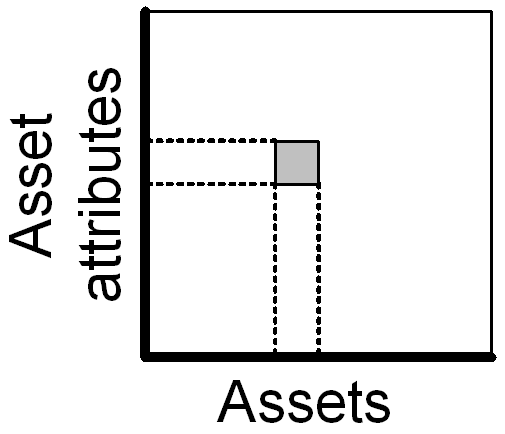
\includegraphics[width=0.25\textwidth]{img/figure1}
\caption{Asset decision sub-space {\textless}sample figure{\textgreater}}\label{fig:1}
\end{figure}
{\textless}Make sure your caption uses the ‘Figure’ style{\textgreater}

\begin{table}[H]
	\centering
	\caption{Software process modeling constructs {\textless}Sample table{\textgreater}}
	\label{tab:01}
	\begin{tabular}{p{0.33\linewidth-2\tabcolsep}p{0.67\linewidth-2\tabcolsep}}
		\toprule
		\multicolumn{1}{c}{\textbf{Modeling construct}} & \multicolumn{1}{c}{\textbf{Description}} \\ \midrule
		Agents & An actor who performs an activity (process element) \\
		Roles & Set of responsibilities assigned to an agent \\
		Artifacts & A product created or maintained by the activities \\
		Activities & Steps that need to achieve process objectives \\
		Tools & Are to be utilizes by the process \\ \bottomrule
	\end{tabular}
\end{table}

{\textless}Make sure your caption uses the ‘Table’ style{\textgreater}

\chapter[CASE STUDY (RESULTS AND DISCUSSION)]{\hfill CHAPTER 4 \hfill\null\vskip15pt CASE STUDY (RESULTS AND DISCUSSION)}

\chapter[CONCLUSIONS]{\hfill CHAPTER 5 \hfill\null\vskip15pt CONCLUSIONS}

{\textless} Did you achieve your objective? Do you have the anticipated deliverable? What did you learn? What do you see for future or additional work?{\textgreater}

\clearpage

\addcontentsline{toc}{chapter}{REFERENCES}
\bibliographystyle{apacite}
\nocite{*}
\bibliography{references}

\backmatter

\chapter[APPENDIX A: USERS’ MANUAL]{\hfill APPENDICES \hfill\null\newline\newline APPENDIX A: USERS’ MANUAL}

{\textless}In the appendices, include such things a users’ manual, program code, diagrams, charts, tables, glossaries, and/or database structures and relationships as well as project management deliverables such as Work Breakdown Structure (WBS) and Gantt Chart.{\textgreater}

\chapter{APPENDIX B: SYSTEM TECHNICAL DOCUMENTATION}

\end{document}
